\paragraph{UC6.4.2 - Selezione della dimensione da associare al colore}
\begin{itemize}
	\item \textbf{Attore primario}: Utente;
	\item \textbf{Precondizioni}: L'utente ha selezionato la visualizzazione \textit{Proiezione Lineare Multi Asse} [UC5.4];
	\item \textbf{Postcondizioni}: L'utente ha associato un colore ai punti del grafico;
	
	\item \textbf{Scenario principale}: L'utente visualizza la lista delle dimensioni, originali o create tramite riduzione dimensionale, del dataset che sta analizzando. Una volta selezionata la voce desiderata, ad ogni punto verrà associato uno specifico colore. 
\end{itemize}

\subsubsection{UC6.5 - Personalizzazione Heat Map}
\begin{figure}[h]
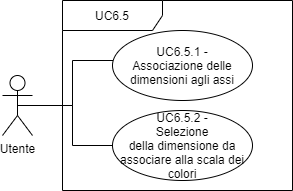
\includegraphics[width=9cm]{Section/Images/UC6.5.png}
\centering
\caption{UC6.5 - Personalizzazione Heat Map}
\end{figure}
\begin{itemize}
	\item \textbf{Attore primario}: Utente;
	
	\item \textbf{Precondizioni}: L'utente ha scelto il grafico \textit{Heat Map} [UC5.5];
	
	\item \textbf{Postcondizioni}: Il grafico viene aggiornato;
	
	\item \textbf{Scenario principale}: L'utente decide:
	
\begin{enumerate}
\item Le dimensioni da associare agli assi del grafico [UC6.5.1];
\item La dimensione da associare alla scala dei colori [UC6.5.2].
\end{enumerate}	
		
\end{itemize}

\paragraph{UC6.5.1 - Associazione delle dimensioni agli assi}
\begin{itemize}
	\item \textbf{Attore primario}: Utente;
	\item \textbf{Precondizioni}: L'utente ha selezionato la visualizzazione \textit{Heat Map} [UC5.5];
	\item \textbf{Postcondizioni}: L'utente ha associato le dimensioni agli assi del grafico;
	
	\item \textbf{Scenario principale}: L'utente visualizza, per ogni asse, tutte le dimensioni del dataset che sta analizzando. Selezionata la voce desiderata, la dimensione verrà associata allo specifico asse del grafico. 
\end{itemize}

\paragraph{UC6.5.2 - Selezione della dimensione d'associare alla scala di colori}
\begin{itemize}
	\item \textbf{Attore primario}: Utente;
	\item \textbf{Precondizioni}: L'utente ha selezionato la visualizzazione \textit{Heat Map} [UC5.5];
	\item \textbf{Postcondizioni}: L'utente ha associato alla scala di colori una dimensione;
	
	\item \textbf{Scenario principale}: L'utente visualizza una lista delle dimensioni del dataset che sta analizzando. Selezionata la voce desiderata, la dimensione verrà associata alla scala di colori del grafico. 
\end{itemize}